\documentclass[tikz]{standalone}
\usepackage{tikz}
\usetikzlibrary{patterns,snakes}
 
\begin{document}
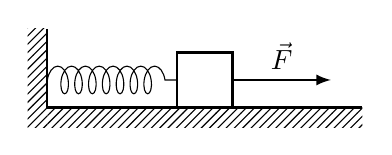
\begin{tikzpicture}

	\draw [draw=none, pattern=north east lines] (0,0) rectangle (4,-0.25);
	\draw [draw=none, pattern=north east lines] (-0.25,1) rectangle (0,-0.25);
	\draw [thick] (0,1) -- (0,0) -- (4,0);
	\draw [thick] (1.65, 0) rectangle (2.35, 0.7);
	\draw [snake=coil, segment amplitude=5pt, segment length=5pt] (0,0.35) -- (1.65, 0.35);
	\draw [arrows={-latex}, thick] (2.35, 0.35) -- (3.6, 0.35) node [midway, above]  {$\vec{F}$};

\end{tikzpicture}
\end{document}